\documentclass[11pt,a4paper]{report}
\usepackage[T1]{fontenc}
\usepackage{graphicx}
\usepackage{amssymb}
\usepackage{xcolor}
\usepackage[hidelinks,colorlinks=true,urlcolor=blue,linkcolor=teal]{hyperref}
\usepackage{minted}
\usepackage[margin=1in]{geometry}
% \usepackage{showframe} % debugging
\usepackage{longtable}
\usepackage{setspace}
\usepackage{mathtools}
\usepackage{makecell}
\usepackage[most]{tcolorbox}
\usepackage{float}
\usepackage{titlesec}
\usepackage{datetime2}

\tcbset{enhanced,colback=white,colframe=cyan!75!black,fonttitle=\bfseries}
\hypersetup{
	pdftitle={CE Lab note},
	pdfsubject={Some theory and MATLAB implementation of various modulation and encoding schemes}
}

\newcommand{\note}[1]{%
	\begin{tcolorbox}[colframe=orange!75!black, title=Note]
		#1
	\end{tcolorbox}
}
\newcommand{\importMLCode}[1]{%
	\setstretch{1}
	\inputminted{matlab}{#1}
	\setstretch{1.15}
}
\renewcommand\cellgape{\Gape[10pt]}

\begin{document}
\setstretch{1.15}
\begin{center}
	{\Huge \normalfont \underline{CE Lab Notes}}
	
	\vspace*{10pt}
	\texttt{Last updated: \today\ \DTMcurrenttime}
	
	\vspace*{10pt}
\end{center}
\titleformat{\chapter}[display]{}{}{}{\bfseries\huge\filcenter}
\titlespacing{\chapter}{0pt}{10pt}{20pt}

\begin{center}
	{\let\clearpage\relax \tableofcontents}
\end{center}

\vspace*{20pt}
\note{These are notes I made along while I was studying for exam (and later refined).
Many implementations done here are directly based on the theory. Hence certain things might be confusing at first.
This is intended as a reference, and defintly not something to mug up night before exam. :)

Also in each program I've put plotting codes inside a function (such as \mintinline{matlab}|plot_sig_fft|, \mintinline{matlab}|plot_|, \texttt{stairz}, etc..)
This is to make code look neater, so that logic of program is not much obstructed by code to plot things
}

\titleformat{\chapter}[frame]
{\huge\fontfamily{qpl}\selectfont}
{\filcenter\enspace \thechapter\enspace}
{10pt} % margin-bottom
{\filcenter}

\chapter{AM modulation and demodulation}
There're 3 types of AM modulation:
\begin{enumerate}
	\item DSBSC
	\item DSBFC
	\item SSBSC
\end{enumerate}

\section{Double Side Band Full carrier: DSBFC}
\setlength{\parindent}{0pt}

For message signal $m(t)$ and carrier $c(t)$, DSBFC is given by:
$$s(t) = (1 + k \times m(t)) c(t)$$

where $k$ is modulation order / modulation index


Demodulation can be done by a \underline{Square law demodulator}. Here modulated wave is squared and passed through a LPF (with cutoff near to message frequency). Additionally DC component can be removed (if needed).

\subsection*{Program}
\importMLCode{code/dsbfc.m}

\begin{figure}[H]
	\centering
	\includegraphics[width=\textwidth]{img/dsbfc.pdf}
\end{figure}

\pagebreak

\section{Double Side Band Suppressed carrier: DSBSC}

Modulation can be done using a \underline{balenced modulator}:

\begin{figure}[H]
	\centering
	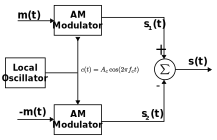
\includegraphics[width=.6\textwidth]{img/balanced_modulator.pdf}
\end{figure}
Hence expression for modulated wave is: 
\begin{align*}
	s(t) &= s_1(t) - s_2(t) \\
	 &= (1 + k \times m(t)) c(t) - (1 - k \times m(t)) c(t) \\
	 s(t)    &= 2k \times m(t) c(t)
\end{align*}

if we ignore $2k$ factor: 
$$s(t) = m(t)c(t)$$


Demodulation can be done by \underline{Coherent detection}: 
\begin{figure}[H]
	\centering
	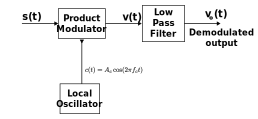
\includegraphics[width=.7\textwidth]{img/coh_detec.pdf}
\end{figure}

Hence demodulated output is: 
$$v_o(t) = \text{LPF}\left[s(t)\cdot c(t)\right]$$

\subsection*{Program}
\importMLCode{code/dsbsc.m}

\begin{figure}[H]
	\centering
	\includegraphics[width=\textwidth]{img/dsbsc.pdf}
\end{figure}

\section{Single Side Band Suppressed carrier: SSBSC}

A reliable Modulation method is  \underline{Frequency Discrimination Method}. This involves shifting phase of message and carrier signals. This can be done manually by writing their expressions, or by using using \href{https://en.wikipedia.org/wiki/Hilbert_transform}{Hilbert transform}.

\begin{figure}[H]
	\centering
	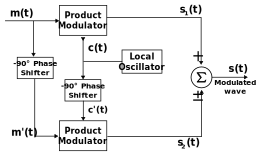
\includegraphics[width=.7\textwidth]{img/freq_disc.pdf}
\end{figure}

\subsection{Case where message and carrier are cos wave}
For a specific case of sine waves: 
if message is $m(t) = A_m \cos\left ( 2 \pi f_mt \right )$ and carrier is $c(t) = A_c \cos\left ( 2 \pi f_ct \right )$.

Product modulator output in top section is:
\begin{align*}
	s_1\left ( t \right )&=A_mA_c \cos \left ( 2 \pi f_mt \right ) \cos\left ( 2 \pi f_ct \right ) \\
	&=\frac{A_mA_c}{2} \left \{ \cos \left [ 2 \pi\left ( f_c+f_m \right )t \right ]+ \cos\left [ 2 \pi\left ( f_c-f_m \right )t \right ] \right \}
\end{align*}

In bottom section the message and the carrier signal are phase shifted by $-90^\circ$ before applying as inputs to the lower product modulator.

Therefore the output of lower product modulator is
\begin{align*}
	s_2\left ( t \right ) &=A_mA_c \cos\left ( 2 \pi f_mt-90^0 \right ) \cos\left (2 \pi f_ct-90^0  \right ) \\
	 &=\frac{A_mA_c}{2} \left \{ \cos \left [ 2 \pi\left ( f_c-f_m \right )t \right ]- \cos\left [ 2 \pi\left ( f_c+f_m \right )t \right ] \right \}
\end{align*}

To get lower sideband Add $s_1(t)$ and $s_2(t)$
\begin{align*}
	s(t) &= s_1(t) + s_2(t) \\
	\Aboxed{s(t)&=A_mA_c \cos \left [ 2 \pi\left ( f_c-f_m \right )t \right ]}
\end{align*}

To get upper sideband subtract $s_2(t)$ from $s_1(t)$
\begin{align*}
	s(t) &= s_1(t) - s_2(t) \\
	\Aboxed{s(t) &=A_mA_c \cos \left [ 2 \pi\left ( f_c+f_m \right )t \right ]}
\end{align*}

\subsection{General case (using Hilbert transform)}
Hilbert transform on a signal $x(t)$ provides $\pm 90^\circ$ phase shift to all frequencies present in the applied signal.
$-90^\circ$ phase shifted version of signal $x(t)$ can be obtained by taking imaginary part of Hilbert transform of the signal:
$$x'(t) = \mathfrak{Im}\{\mathcal{H}(x(t))\}$$

Hence the $s_2(t)$ can be written in terms of Hilbert transform as :
\begin{align*}
	s_2(t) &= \mathfrak{Im}\{\mathcal{H}(m(t))\}\times \mathfrak{Im}\{\mathcal{H}(c(t))\} \\
\end{align*}
From this lower side band can be obtained as:
$$s_{\text{LSB}}(t) = s_1(t) + s_2(t)$$
And upper side band can be obtained as:
$$s_{\text{USB}}(t) = s_1(t) - s_2(t)$$

\subsection{Demodulation}
Demodulation can be done by a coherent detector:
\begin{figure}[H]
	\centering
	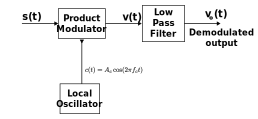
\includegraphics[width=.7\textwidth]{img/coh_detec.pdf}
\end{figure}

\subsection*{Program (with Hilbert transform)}
Here I have demodulated the lower sideband. To get best result, cutoff frequency should be between $2f_m$ and $f_c$.

Message signal here is: $m(t) = 2\sin(2\pi f_m t^2);$
\importMLCode{code/ssbsc.m}

\begin{figure}[H]
	\centering
	\includegraphics[width=\textwidth]{img/ssbsc.pdf}
\end{figure}

\pagebreak
\chapter{FM modulation and demodulation}
\section{Modulation}
For a message signal $m(t)$ and carrier $c(t) = A_c \cos(2\pi f_c t)$ the modulated wave is:
\begin{equation*}
s (t) = A_c \cos\left(2\pi f_c t + 2\pi k_f \int_{0}^{t} m(\tau) d\tau\right)
\end{equation*}
Where $k_f$ is known as \textit{frequency sensitiviy}.
In the case of single tone modulation, where $m(t) = A_m \cos(2\pi f_m t)$ or $m(t) = A_m \sin(2\pi f_m t)$ :

\begin{align*}
	s (t) &= A_c \cos\left(2\pi f_c t + 2\pi k_f \int_{0}^{t} A_m\cos(2\pi f_m \tau) d\tau\right) \\
	&= A_c \cos\left(2\pi f_c t + \frac{2\pi k_f A_m}{2\pi f_m} \sin(2\pi f_m \tau) \right) \\
	s(t) &= A_c \cos\left(2\pi f_c t + \frac{k_f A_m}{f_m} \sin(2\pi f_m \tau) \right)
\end{align*}

Here $k_f A_m = \Delta f$ is called  \textit{frequency deviation} and $\dfrac{k_f A_m}{f_m} = \dfrac{\Delta f}{f_m} = \beta$ is called modulation index.

For a general message signal $m(t)$, modulation index can be defiend as (as far as I looked up in various sources):

$$\beta = \frac{k_f\cdot m_{peak}}{f_{max}}$$

where $f_{max}$ is maximum frequency component present in the message signal. And $m_{peak}$ is peak value of input signal:
$$m_{peak} = \frac{\max\left[m(t) \right] - \min\left[m(t) \right]}{2}$$
You can see that for a simple sine wave with amplitude $A_m$ this just reduces to $m_{peak} = A_m$.

\note{There are some differences in how $\beta$ is defined in various sources.
Here, I've used one of such definitions. (see \textit{page 212, Modern Digital and Analog Communication Systems, B.P. Lathi})}

\section{Demodulation}
Demodulation is done by finding Hilbert transform of FM, extracting instantaneous phase from it and differentiating it (minus phase offset due to carrier):
Hilbert transform: 
$$z = \mathcal{H}(s(t))$$
Instantaneous phase angle (obtained by \mintinline{matlab}|unwrap(angle(z))|)
$$\theta(t) = \measuredangle z(t)$$

Demodulated wave is:
$$m'(t) = \frac{\partial}{\partial t} (\theta(t) - 2 \pi f_c t)$$

\section{Program for narrow and wide band FM modulation and demodulation}
Narrow band FM has $\beta << 1$ and wide band FM has $\beta >> 1$

To modulate at a particular value of $\beta$, $k_f$ has to be found out first
$$k_f =\frac{\beta f_{max}}{m_{peak}}$$

But i don't think, this level of perfection is required in lab exam - they didnt ask for details of how it was implemented.
In the program I've done this anyway. To integrate message signal cumulative summer \mintinline{matlab}|cumsum(m)| is used.

The message signal chosen here is: $m(t) = \sin(2 \pi f_m t) + \sin(4 \pi f_m t)$. Here $f_{max} = 2f_m$.

\importMLCode{code/fm_mod.m}

\begin{figure}[!ht]
	\centering
	\includegraphics[width=\textwidth]{img/fm.pdf}
\end{figure}

\pagebreak
\chapter{PAM modulator and demodulator}

PAM modulation is done by multiplying a square wave by message signal.
\textit{The minimum amplitude of square wave should be 0}, which can be either constructed by \texttt{square} or \texttt{sin} function:
\begin{itemize}
	\item \texttt{sin(2 * pi * fc * t) > 0}
	\item \texttt{square(2 * pi * fc * t) > 0}
\end{itemize}

% \section{Demodulation}
% Demodulation can be done in 2 ways: cumulatI'vesummer and low pass filter.
% \subsection{Low pass filter}

% For perfect integration: $RC > 15T$ where $T=1/f$

% If the frequency of clock is f = 1 KHz

% $$RC > \frac{15}{1kHz}$$

% Let $C = 1\uf$, then 

% \begin{align*}
% 	R &> \frac{15}{1kHz * 1\uf} \\
% 	R &> 1.5k\ohm
% \end{align*}

% in fact any value of $R > 1.5k\ohm$ will work. But more the value of $R$, more will be the attenuation
% \subsection{CumulatI'vesummer}

Demodulation is done by a passing PAM wave to low pass filter with cut off frequency slightly higher than highest frequency in the message signal.
\section*{Program}
Here message is $m(t) = 0.5\sin(2\pi f_m t) + \sin(6\pi f_m t)$

\importMLCode{code/pam_exp.m}

\begin{figure}[!ht]
	\centering
	\includegraphics[width=\textwidth]{img/pam.pdf}
\end{figure}

\pagebreak
\chapter{Binary Shift Keying}

Orthonormal carrier signals in each modulation scheme are: \\[10pt]

\newcommand{\se}{\sqrt{\dfrac{2E_b}{T_b}}}

\begin{center}
	\begin{tabular}{|c|c|}
\hline
BASK & \makecell{$\begin{aligned}
s_1(t) &= \se \cos(2\pi f_c t) \\[10pt]
s_2(t) &= 0
\end{aligned}$} \\ \hline
BPSK & \makecell{$\begin{aligned}
	s_1(t) &= \se \cos(2\pi f_c t) \\[10pt]
	s_2(t) &= \se \cos(2\pi f_c t + \pi)
\end{aligned}$} \\ \hline
BFSK & \makecell{$\begin{aligned}
	s_1(t) &= \se \cos(2\pi f_{c1} t) \\[10pt]
	s_2(t) &= \se \cos(2\pi f_{c2} t)
\end{aligned}$} \\ \hline
\end{tabular}
\end{center}
Transmitted wave is given by

\begin{equation*}
s(t) = \begin{cases}
		s_1(t)  &  \text{if bit = 1} \\
		s_2(t)  &  \text{if bit = 0}
	\end{cases}
\end{equation*}
For demodulation, refer: \nameref{mary}

Throughout the entire program (and in other programs like line codes, etc), I've used \texttt{kron} function. more on that function below:
\section*{\texttt{kron} function \label{kronfx}}
\texttt{kron} is used to implement \href{https://en.wikipedia.org/wiki/Kronecker_product}{Kronecker product} which is here used to create copies of a carrier signal based on the message signal.
Kronecker product of two matricies $A = \begin{bmatrix}1 & 2 & 3\end{bmatrix}$ and $B = \begin{bmatrix}1 & 1 & 0 & 0\end{bmatrix}$ is:

$$\begin{aligned}
	A \otimes B &= \begin{bmatrix}1 & 2 & 3\end{bmatrix} \otimes \begin{bmatrix}1 & 1 & 0 & 0\end{bmatrix} \\
&= \begin{bmatrix}
1 \begin{bmatrix}1 & 1 & 0 & 0\end{bmatrix} & 
2 \begin{bmatrix}1 & 1 & 0 & 0\end{bmatrix} & 
3 \begin{bmatrix}1 & 1 & 0 & 0\end{bmatrix}
\end{bmatrix} \\
&= \left[\begin{array}{cccccccccccc}
	1 & 1 & 0 & 0 & 2 & 2 & 0 & 0 & 3 & 3 & 0 & 0
\end{array}\right]
\end{aligned}
$$

From this you can see \texttt{kron} can produce any required copies of a carrier signal based on message bit stream:

\begin{figure}[!ht]
	\centering
	\includegraphics[width=\textwidth]{img/kron.pdf}
\end{figure}

This function is used extensively throughout the remaining MATLAB codes in this PDF.

\section*{Program}
\importMLCode{code/bsk.m}

\begin{figure}[!ht]
	\centering
	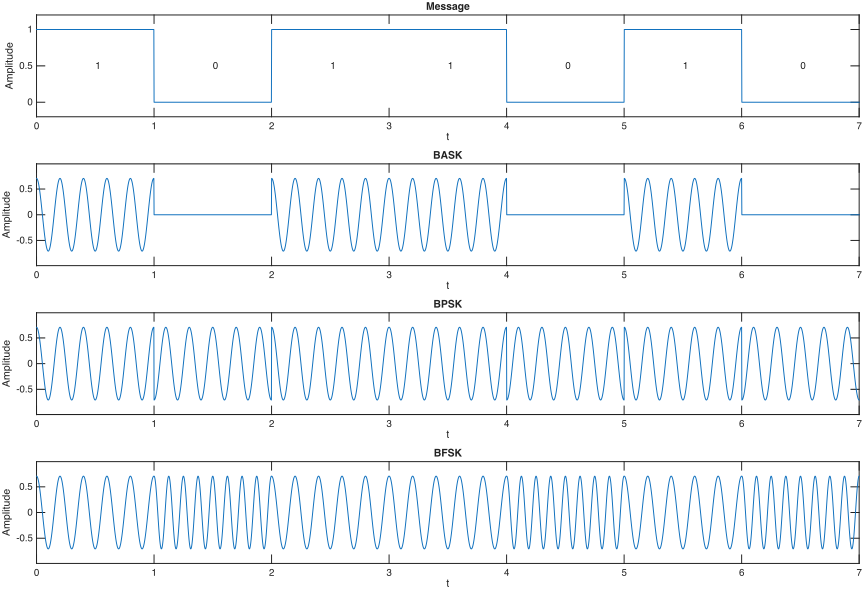
\includegraphics[width=\textwidth]{img/bsk.pdf}
\end{figure}



\chapter{Line Codes}
\setlength{\parindent}{0pt}
There are many line coding methods, Few of them are:

\begin{enumerate}
	\item Non-Polar Return to Zero (NPRZ)
	\item Non-Polar Non Return to Zero (NPNRZ)
	\item Polar Return to Zero (PRZ)
	\item Polar Non Return to Zero (PNRZ)
	\item Manchester
	\item Bipolar
	\item Differential
\end{enumerate}
To encode a input bitstrean $x(n)$, over a symbol period $T_b$,
following expression are used to generate the required line code sequence.

\begin{longtable}{|r|l|}
	\hline
	NPRZ & \makecell[l]{$s(t) = \begin{cases}
		1  & \text{if }x(n) = 1 \\
		0  & \text{if }x(n) = 0
	\end{cases}\quad $ For entire bit interval} \\ \hline
	
	NPNRZ & \makecell[l]{
		for $x(n) = 1$, $s(t) = \begin{cases}
		1  & 0 \le t \le \frac{T_b}{2} \\
		0  & \frac{T_b}{2} < t \le T_b
	\end{cases}\vspace*{5pt}$ \\
	for $x(n) = 0, s(t) = 0$} \\ \hline
	
	PRZ & \makecell[l]{$s(t) = \begin{cases}
		1  & 0 \le t \le \frac{T_b}{2} \quad \text{for } x(n) = 1 \\
		-1  & 0 \le t \le \frac{T_b}{2} \quad \text{for } x(n) = 0 \\
		0  & \frac{T_b}{2} < t \le T_b
	\end{cases}$}\\ \hline
	
	PNRZ & \makecell[l]{$s(t) = \begin{cases}
		1  & \text{if } x(n) = 1 \\
		-1  & \text{if } x(n) = 0
	\end{cases} \quad \text{For entire bit interval}$}  \\ \hline
	
	\makecell[r]{Manchester  \\ (\href{https://en.wikipedia.org/wiki/Manchester_code\#Encoding_and_decoding}{IEEE 802.3})} & \makecell[l]{for $x(n) = 0 \quad s(t) = \begin{cases}
		1  & 0 \le t \le \frac{T_b}{2} \\
		-1  & \frac{T_b}{2} < t \le T_b
	\end{cases}\vspace*{10pt}$ \\
	for $x(n) = 1 \quad s(t) = \begin{cases}
		-1  & 0 \le t \le \frac{T_b}{2} \\
		1  & \frac{T_b}{2} < t \le T_b
	\end{cases}$} \\ \hline
	
	Bipolar & \makecell[l]{for $x(n) = 0$, $s(t) = 0$ \\
	for $x(n) = 1$, $s(t) = 1\text{ or }-1$\ alternatively
	} \\ \hline
	
	Differential &  \makecell[l]{$s(n) = x(n) \odot s(n-1)\quad $ (xnor operation)} \\
	\hline
\end{longtable}

\section*{Program}
Here bipolar and differential line code output are lists with same number of elements as that of input bitstrean.
This is because i haven't sampled them like other codes, (but you can sample them, using \texttt{kron} or in other ways).

\importMLCode{code/linecode.m}

For the purpose of getting nice plot, x axis of all plots starts from 1 (can you guess why?)

\begin{figure}[!ht]
	\centering
	\includegraphics[width=0.9\linewidth]{img/linecode.pdf}
\end{figure}
\chapter{M-ary modulation schemes}
\label{mary}
In the following programs, I've implemented a general M-ary shift keying modulator.
So to get 4-ary modulation (or 8-ary) just set $M$ = 4 (or $M$ = 8) in the program.

\section{Context}
An M-ary modulation means, for modulating quantity, M different level are used for transmitting M symbols.
\begin{itemize}
	\item in M-ary FSK: M different frequencies are used.
	\item in M-ary PSK: M different phases are used.
	\item in M-ary ASK: M different amplitudes are used.
\end{itemize}

Usually all these modulated quantities are equally spaced.

When a bit sequence is given, they have to be grouped and converted to equivalent decimal format to do rest of modulation.
For M-ary modulation, number of bits in each group is $n = log_2(M)$.
If Enough bits are not there (ie we have to group every 2 bits, but there're only 5 bits), additional zeros has to added. For eg. grouping in 4-ary will be:

00101 -> 00 10 10 (grouping of 2 bits)

and in 8-ary:

00101 -> 001 010 (grouping of 3 bits)

Where the zero should be added?
It cab be added in either front or back of the sequence, as long as you can create a demodulate scheme which discards this extra zero.
(in this case I've added it at the end of each group).

\section{M-ary ASK}
Generally for M signals, M different amplitude levels should be used.
For eg. in QASk, 4 equally spaced amplitude levels will be used. In practice, it can be of any value: [1 2 3 4] or [-3 -1 1 3], etc...

In my implementation, I created amplitude levels corresponding to each decimal digit $d$ which ranges from 0 to $M-1$ by interpolating $d$ to range from $L_{min}$ to $L_{max}$
(which corresponds to minimum and maximum amplitude level). Hence amplitude corresponds to decimal digit $d$ is

$$\therefore \text{amplitude(d)} = \frac{d}{M-1} * (L_{max} - L_{min}) + L_{min}$$

\subsection*{Program}
\setstretch{1}
\importMLCode{code/mary.m}
\setstretch{1.15}
The length of sequnce has to be adjusted in such a way that grouping is possible. for 4-ary, input length should be multiple of 2, for 8-ary, input length should be multiple of 3, and so on..

To do such adjustment, some number of bits should be added. The following code checks if input length is multiple of $n$ and if not, it adds required number of zeros.
\begin{minted}[frame=single]{matlab}
if mod(length(x), n) ~= 0
    x = [x, zeros(1, n - mod(length(x), n))];
end
\end{minted}

for eg.: if n = 3 (for 8-ary modulation), and input length is 7, {\tt mod(7, 3) = 1}, hence 3 - 1 = 2 more zeros are added.

\begin{figure}[ht!]
	\centering
	\includegraphics[width=\textwidth]{img/mask.pdf}
\end{figure}


\section{M-ary PSK}
M-ary here divides phases from 0 to $2\pi$ into M intervals.
If each group of bits corresponds to digit d. Then corresponding M-PSK signal is:
$$s(t) = A_c \sin\left(2 \pi f_c t + \frac{2\pi}{M} d\right)$$

Where $d$ can take valus either from 0 to $M-1$ or 1 to $M$. Notice that in this representation the signal constellation will contain a signal vector at $0^\circ$. This signal vector at $0^\circ$ can be avoided by adding additional phase shift of $\pi / M$ to whole signal. This is illustrated in following:
\\[10pt]
\begin{figure}[!ht]
	\begin{minipage}[t]{.45\textwidth}
		\centering
		\includegraphics[width=\linewidth]{img/0ps.pdf}
\\[10pt]
		With signal vector at $0^\circ$ \\[5pt]
		$s(t) = A_c \sin\left(2 \pi f_c t + \dfrac{2\pi}{M} d\right)$
	\end{minipage}\hfill%
	\begin{minipage}[t]{.45\textwidth}
		\centering
		\includegraphics[width=\linewidth]{img/ps.pdf}
\\[10pt]
		No signal vector at $0^\circ$ \\[5pt]
		$s(t) = A_c \sin\left(2 \pi f_c t + \dfrac{2\pi}{M} d + \dfrac{\pi}{M}\right)$
	\end{minipage}
\end{figure}

\subsection*{Program}
Here I've implemented a modulator that doesn't produce signal vector at $0^\circ$ phase shift. Here's how it is implemented:

I've expressed all signals in complex form, this allows phase shift to be applied to signals by just multiplying by another complex number.
The carrier signal is written in complex form:
$$c(t) = A_c\exp\left(j2\pi f_c t\right)$$

Phase shift for a partial symbol $d$ is:
\begin{equation}
	\text{phase}(d) = \exp\left[j\left(2\pi \dfrac{d}{M} + \dfrac{\pi}{M}\right)\right]
	\label{phased}
\end{equation}

Hence signal corresponding to given decimal $d$ is:
\begin{align*}
	s(t) &= c(t) \cdot \text{phase}(d) \\
&= A_c\exp\left(j2\pi f_c t\right) \exp\left[j\left(2\pi \dfrac{d}{M} + \dfrac{\pi}{M}\right)\right] \\[5pt]
\Aboxed{s(t)&= \exp\left[j\left(2\pi f_c t + 2\pi \dfrac{d}{M} + \dfrac{\pi}{M}\right)\right]}
\end{align*}

To plot the signal, either real or imaginary part of $s(t)$ can be taken.
If imaginary part is taken:

$$\mathfrak{Im}(s(t)) = A_c\sin\left[2\pi f_c t + 2\pi \dfrac{d}{M} + \dfrac{\pi}{M}\right]$$

NOTE: in the program, $A_c$ is taken as 1.
\importMLCode{code/mpsk.m}

\begin{figure}[!ht]
	\centering
	\includegraphics[width=\linewidth]{img/mpsk.pdf}
\end{figure}

The signal constellation will have axis which are orthonormal basis functions used in PSK. 
Here, I've used \textit{orthogonal} signals: $s1(t) = \cos(2\pi f_c t)$ and $s2(t) = \sin(2\pi f_c t)$
which are real and imaginary component of phase(d) in Eq. \ref{phased}.

The case illustrated above is 4-ary. If you want to plot constellation for 8-ary, appropriate message bit stream must be provided, that generates signals of all phases (this is true for all other modulation schemes)

\section{M-ary FSK}

In the same way, M-ary FSK will have M different frequencies: $$f_c, \quad f_c + \Delta f, \quad f_c + 2\Delta f, \quad \cdots, \quad f_c + (M-1)\Delta f$$

Where $\Delta f$ is the distance between each frequency.

Hence for each decimal digit $d$ corresponding to some group of binary, signal is given by:

$$s(t) = \sin\left(2\pi (f_c + d \Delta f) t\right)$$

\subsection*{Program}
\importMLCode{code/mfsk.m}
\begin{figure}[!ht]
	\centering
	\includegraphics[width=0.8\linewidth]{img/mfsk.pdf}
\end{figure}

The signal constellation of M-ary FSK will have M-dimensions, which is hard to visualize for 4-ary or 8-ary FSK.

\section{BER vs SNR, Signal constellation}
The following is an example for BER(Bit error rate) or Symbol error rate (for M-ary modulation) vs SNR plot of BPSK and QPSK. BER is ratio of number of wrong symbols detected after demodulation to total number of symbols. Usually its a small number hence it is expressed in log scale:

$$\text{BER} = 10\log_{10} \left(\frac{\text {No. of incorrectly decoded symbols}}{\text{Total no. of symbols}}\right)$$

The errors can happen due to noise in the channel.
This noise is simulated by using function \texttt{awgn(x, snr)} .
This function adds noise to input $x$ in such a way that the output SNR is as given to it.
Hence to obtain BER at a given \texttt{snr} following steps are done: (this is same for any modulation scheme)
\begin{enumerate}
	\item Modulate signal $x(n)$ and obtain $m(t)$ (modulated wave)
	\item apply noise: \mintinline{matlab}{y = awgn(x, snr)} 
	\item demodulate it, and get $d(n)$
	\item Count number of symbol errors (using \mintinline{matlab}{sum(x ~= d)})
\end{enumerate}

{\setlength{\parindent}{0pt} Use a loop to find BER for a range of SNRs}

\subsection*{Program}
This uses matlab's built in \mintinline{matlab}{pskmod} and \mintinline{matlab}{pskdemod} functions.


\importMLCode{code/psk_ber.m}

\begin{figure}[!ht]
	\centering
	\includegraphics[width=\linewidth]{img/psk_perf.pdf}
\end{figure}

\begin{tcolorbox}[breakable, title=More on Matlab's build-in modulators \& demodulators]
	In my implementation, I took a bit sequence and converted it to decimal to do any useful operation. However MATLAB's build in functions only takes decimal values. The modulation also works differently (for eg: in case of PSK, matlab uses gray codes to map each input to corresponding phase value, also it uses different set of phase differences). If you try with PSK, you'll get following points: 
\begin{minted}[frame=single]{matlab}
>> pskmod([0 1 2 3], 4)
ans =
1.0000 + 0.0000i
0.0000 + 1.0000i
-0.0000 - 1.0000i
-1.0000 + 0.0000i

>> pskmod([0 1 2 3 4 5 6 7], 8)
ans =
1.0000 + 0.0000i
0.7071 + 0.7071i
-0.7071 + 0.7071i
0.0000 + 1.0000i
0.7071 - 0.7071i
-0.0000 - 1.0000i
-1.0000 + 0.0000i
-0.7071 - 0.7071i
\end{minted}

This is visualised as following: (notice that grey code is assigned in clockwise manner)

\begin{minipage}[t]{\textwidth}
		\centering
		\includegraphics[width=0.9\linewidth]{img/psk_diag.pdf}
\end{minipage}

Subsequently, the demodulation also produces integer sequence corresponding to each modulated vector.

\begin{minted}[frame=single]{matlab}
>> pskdemod([1, i, -i, -1], 4)
ans =
0     1     2     3
\end{minted}

Similarly there is \texttt{fmmod} and \texttt{fmdemod} functions for FM modulation. More on it here:
\href{https://in.mathworks.com/help/comm/ref/fmmod.html}{https://in.mathworks.com/help/comm/ref/fmmod.html}
	
\end{tcolorbox}


\end{document}